\section{Exercise one}

Consider the stochastic process defined by the following diagram:
\begin{figure}[H]
    \centering
    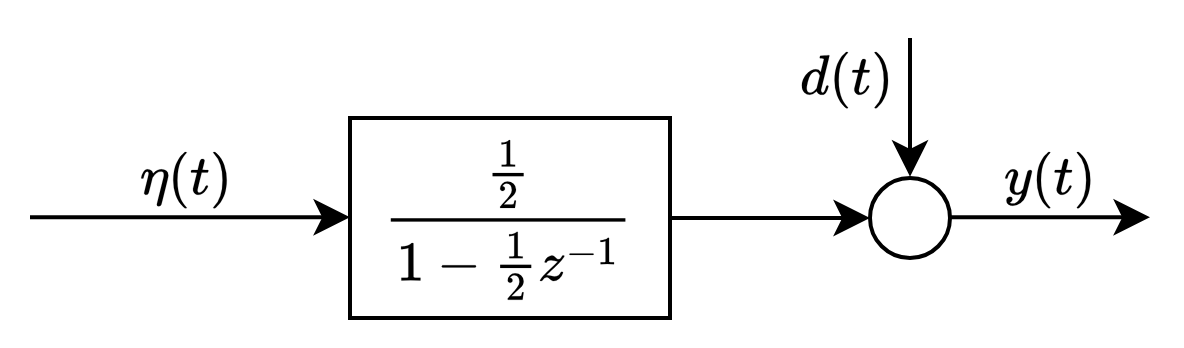
\includegraphics[width=0.5\linewidth]{images/21.png}
\end{figure}
Where: 
\begin{itemize}
    \item $v(t) = \dfrac{1}{2} v(t-1) + \dfrac{1}{2} \eta(t) \quad \eta(\cdot) \sim WN(0, 1)$.
    \item $d(\cdot) \sim WN(0, 1) $.
    \item $\eta(\cdot)$ and $d(\cdot)$ are two independent white processes (uncorrelated).
\end{itemize}
Calculate the spectrum of process $y(\cdot)$.

Now consider that $d(t) = \eta(t)$ and compute the spectrum.

\subsection{Solution}
Let's compute the expected value of the process:
\[\mathbb{E}\left[ y(t) \right]=0\]
Because it is the sum of two processes with expected values equal to zero.

Now we compute the covariance at a generic time instant $\tau$:
\begin{align*}
    \gamma_y(\tau)  &= \mathbb{E}\left[\left(v(t)+d(t)\right)\left(v(t+\tau)+d(t+\tau)\right)\right] \\
                    &= \mathbb{E}\left[v(t)v(t+\tau) + v(t)d(t+\tau) + d(t)v(t+\tau) + d(t)d(t+\tau)\right] \\
                    &= \underbrace{\mathbb{E}\left[v(t)v(t+\tau)\right]}_{\gamma_v(\tau)}  + \underbrace{\mathbb{E}\left[v(t)d(t+\tau)\right]}_{\eta \bot d}  + \underbrace{\mathbb{E}\left[d(t)v(t+\tau)\right]}_{\eta \bot d}  + \underbrace{\mathbb{E}\left[d(t)d(t+\tau)\right]}_{\gamma_d(\tau)}  \\
                    &= \gamma_v(\tau) + \gamma_d(\tau) \\
\end{align*}
At this point, we have:
\[\Gamma_y(\omega)=\sum_{-\infty}^{\infty}\gamma_y(\tau)e^{-j\omega\tau}=\sum_{-\infty}^{\infty}\gamma_v(\tau)e^{-j\omega\tau} + \sum_{-\infty}^{\infty}\gamma_d(\tau)e^{-j\omega\tau}=\Gamma_v(\omega)+\Gamma_d(\omega) \]
So, we can obtain the spectrum as the sum of the spectra of the two processes: 
\begin{align*}
    \Gamma_y(\omega)    &=\left\lvert W(e^{j\omega}) \right\rvert^2\cdot\underbrace{\lambda_\eta^2}_1 + \underbrace{\lambda_d^2}_1 \\
                        &=\left\lvert W(e^{j\omega}) \right\rvert^2 + 1 \\
                        &= \dfrac{\frac{1}{4}}{\left\lvert 1-\frac{1}{2}e^{-j\omega} \right\rvert^2} + 1\\
                        &= \dfrac{\frac{1}{4}}{\left\lvert 1-\frac{1}{2}\cos(\omega)+j\frac{1}{2}\sin(\omega)\right\rvert^2} + 1\\
                        &= \dfrac{\frac{1}{4}}{\left(1-\frac{1}{2}\cos(\omega)\right)^2 + \left(\frac{1}{2}\sin(\omega)\right)^2} + 1 \\
                        &= \dfrac{\frac{1}{4}}{\frac{5}{4} - \cos(\omega)} + 1 \\     
                        &= \dfrac{6-4\cos(\omega)}{5-4\cos(\omega)}\\                          
\end{align*}
This result in the following graph: 
\begin{figure}[H]
    \centering
    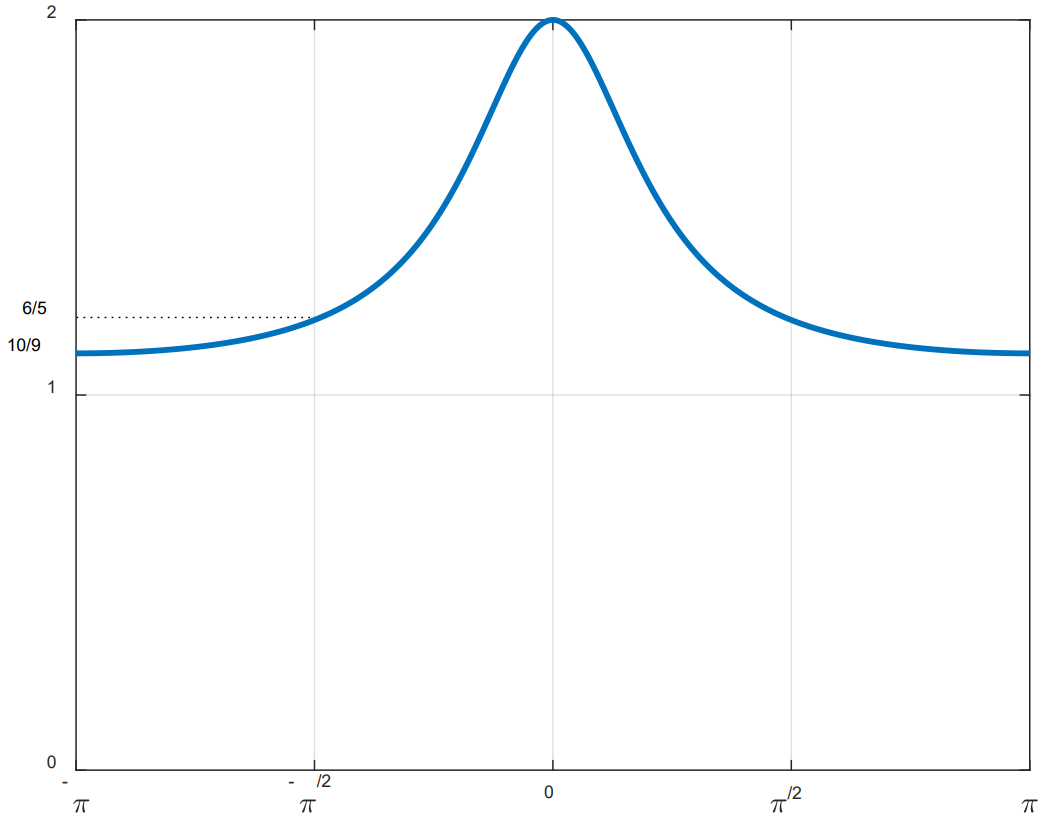
\includegraphics[width=0.5\linewidth]{images/21spec.png}
\end{figure}

In the second case the white noises are correlated, so we have the following block diagram: 
\begin{figure}[H]
    \centering
    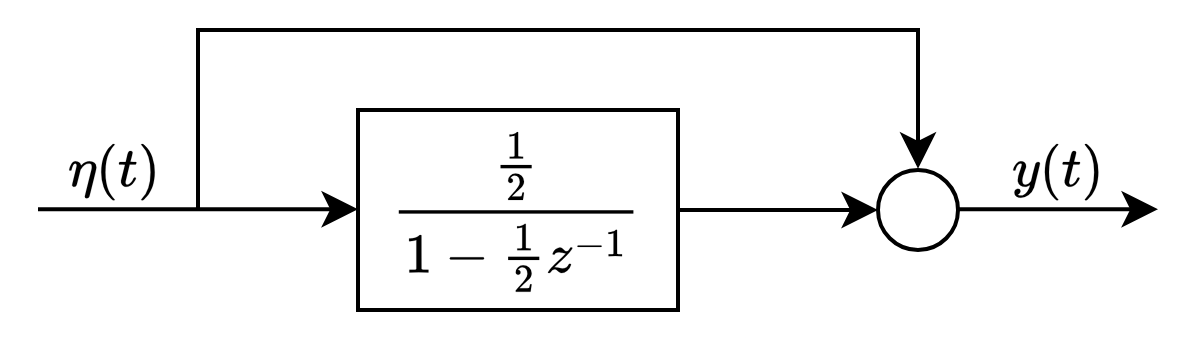
\includegraphics[width=0.5\linewidth]{images/21block.png}
\end{figure}
And the transfer function from $\eta(\cdot)$ to $y(\cdot)$ equals:
\[W(z)=\dfrac{\frac{1}{2}}{1-\frac{1}{2}z^{-1}}+1=\dfrac{\frac{3}{2}-\frac{1}{2}z^{-1}}{1-\frac{1}{2}z^{-1}}\]
The spectrum would be: 
\begin{align*}
    \Gamma_{yy}(\omega) &=\left\lvert W(e^{j\omega}) \right\rvert^2\lambda_n^2 \\
                        &=\left\lvert W(e^{j\omega}) \right\rvert^2 \\
                        &=\dfrac{10-6\cos(\omega)}{5-4\cos(\omega)}
\end{align*}
This result in the following graph: 
\begin{figure}[H]
    \centering
    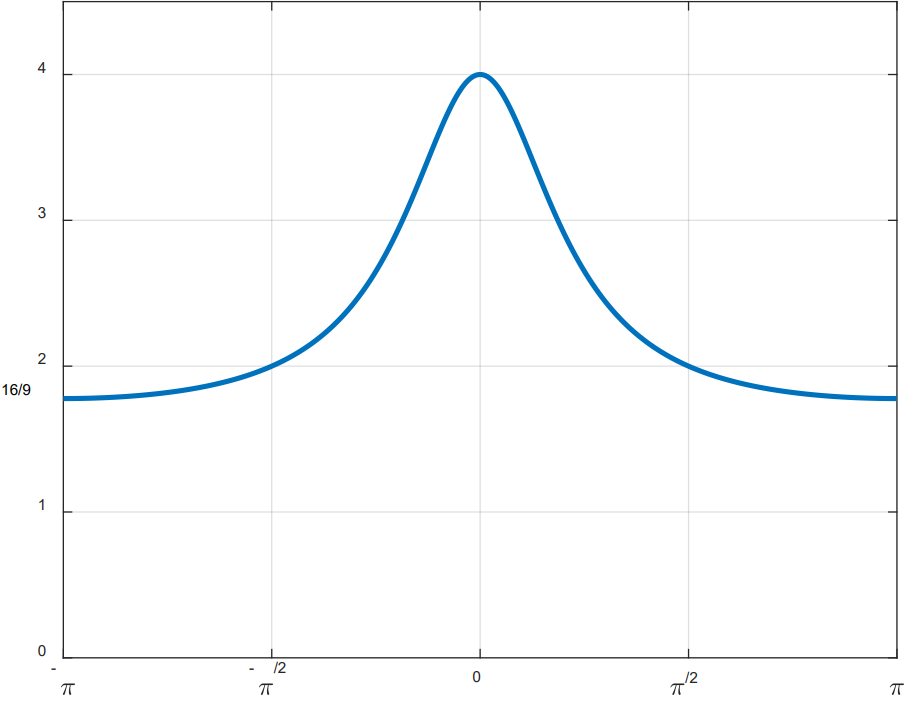
\includegraphics[width=0.5\linewidth]{images/21spec1.png}
\end{figure}